

% ------------------------------



  \begin{figure}[!h]
	  \centering
	  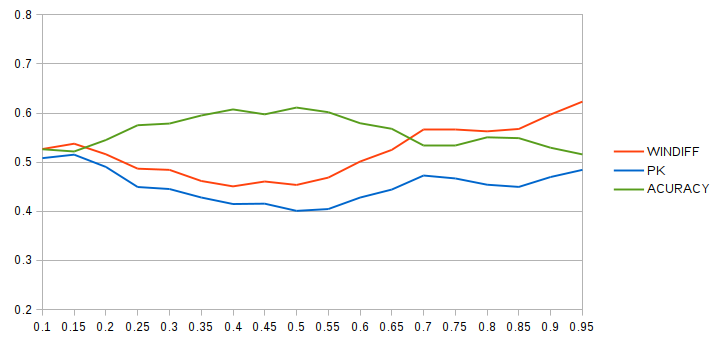
\includegraphics[width=1\textwidth]{conteudo/capitulos/figs/graficos/analiseNSegRate-MinCut.png}
	  \caption{Performance dos algoritmos de segmentação textual}
	  \label{fig:grafico-medidas-tradicionais}
  \end{figure}


  \begin{figure}[!h]
	  \centering
	  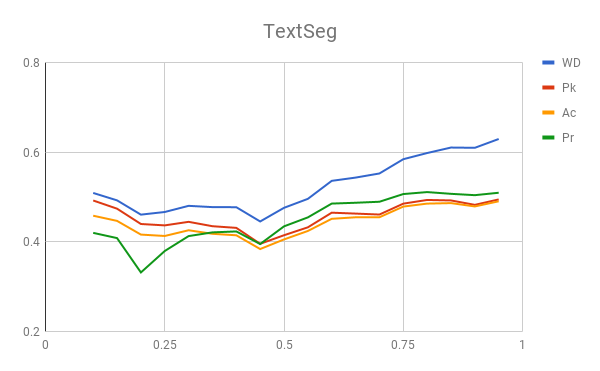
\includegraphics[width=1\textwidth]{conteudo/capitulos/figs/graficos/analiseNSegRate-UISeg.png}
	  \caption{Performance dos algoritmos de segmentação textual}
	  \label{fig:grafico-medidas-tradicionais}
  \end{figure}

  \begin{figure}[!h]
	  \centering
	  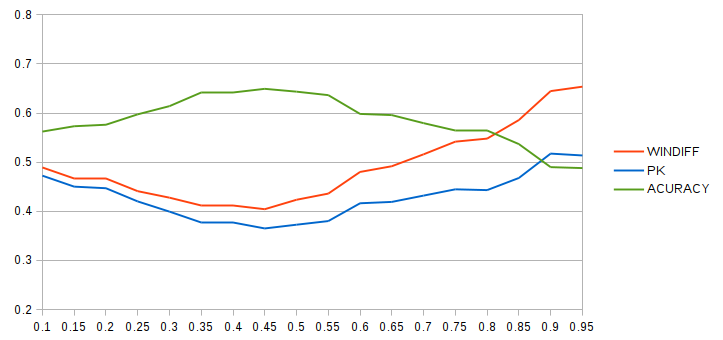
\includegraphics[width=1\textwidth]{conteudo/capitulos/figs/graficos/analiseNSegRate-Bayes.png}
	  \caption{Performance dos algoritmos de segmentação textual}
	  \label{fig:grafico-medidas-tradicionais}
  \end{figure}

  
  \begin{figure}[!h]
	  \centering
	  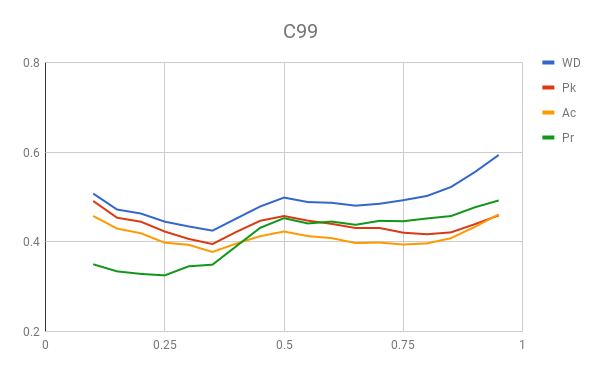
\includegraphics[width=1\textwidth]{conteudo/capitulos/figs/graficos/analiseNSegRate-C99.png}
	  \caption{Performance dos algoritmos de segmentação textual}
	  \label{fig:grafico-medidas-tradicionais}
  \end{figure}


  
  \begin{figure}[!h]
	  \centering
	  \includegraphics[width=1\textwidth]{}
	  \caption{Performance dos algoritmos de segmentação textual}
	  \label{fig:grafico-medidas-tradicionais}
  \end{figure}



% ------------------------------



\begin{table}[!h]
	\centering
	\begin{tabular}{|l||c|c|c|c|c|c|c|c|c|c|c|} \hline

		\textbf{Algoritmo} && 
		\textbf{Step} &
		\textbf{Win} & 
		\textbf{P$_k$} & 
		\textbf{WD} & 
		\textbf{Ac} & 
		\textbf{Pr} & 
		\textbf{Re} &
		\textbf{F$^1$} &
		\textbf{\#Segs} \\	\hline

TextTiling && 20 & 30 & 0.461 & 0.444 & 0.581 & 0.560 & \cellcolor{gray!20} \textbf{0.336} & \cellcolor{gray!20} \textbf{0.411} & 8.833  \\ \hline 
TextTiling && 30 & 45 & \cellcolor{gray!20} \textbf{0.450} & \cellcolor{gray!20} \textbf{0.435} & \cellcolor{gray!20} \textbf{0.596} & \cellcolor{gray!20} \textbf{0.696} & 0.275 & 0.373 & 6.417  \\ \hline 

\hline
		\textbf{Algoritmo} &
		\textbf{RS} &
		\textbf{W} & 
		\textbf{SRate}& 
		\textbf{P$_k$} & 
		\textbf{WD} & 
		\textbf{Ac} & 
		\textbf{Pr} & 
		\textbf{Re} &
		\textbf{F$^1$} &
		\textbf{\#Segs} \\	\hline

C99 & 3 & true  &0.300 &  \cellcolor{gray!20} \textbf{0.434} & \cellcolor{gray!20} \textbf{0.407} & 0.607 & 0.655 & 0.376 & 0.457 & 9.250  \\ \hline 
C99 & 3 & true  &0.700 &  0.485 & 0.431 & 0.602 & 0.553 & \cellcolor{gray!20} \textbf{0.797} & \cellcolor{gray!20} \textbf{0.633} & 21.417  \\ \hline 
C99 & 5 & true  &0.500 &  0.460 & 0.421 & \cellcolor{gray!20} \textbf{0.609} & 0.580 & 0.600 & 0.571 & 15.500  \\ \hline 
C99 & 3 & false &0.200 &  0.448 & 0.427 & 0.596 & \cellcolor{gray!20} \textbf{0.719} & 0.257 & 0.362 & 6.083  \\ \hline 


\hline
		\textbf{Algoritmo} && 
		\textbf{Cut} & 
		\textbf{SRate} &
		\textbf{P$_k$} & 
		\textbf{WD} & 
		\textbf{Ac} & 
		\textbf{Pr} & 
		\textbf{Re} &
		\textbf{F$^1$} &
		\textbf{\#Segs} \\	\hline


MinCutSeg && 13 & 0.300 & 0.457 & 0.427 & 0.594 & \cellcolor{gray!20} \textbf{0.638} & 0.353 & 0.433 & 8.667  \\ \hline 
MinCutSeg && 9  & 0.400 & \cellcolor{gray!20} \textbf{0.444} & 0.408 & \cellcolor{gray!20} \textbf{0.614} & 0.629 & 0.494 & 0.526 & 11.917  \\ \hline 
MinCutSeg && 11 & 0.500 & 0.459 & \cellcolor{gray!20} \textbf{0.407} & 0.603 & 0.588 & 0.590 & 0.563 & 15.000  \\ \hline 
MinCutSeg && 5  & 0.700 & 0.528 & 0.438 & 0.567 & 0.536 & \cellcolor{gray!20} \textbf{0.746} & \cellcolor{gray!20} \textbf{0.599} & 21.000  \\ \hline 


\hline
		\textbf{Algoritmo} &
		\textbf{Prior} &
		\textbf{Disp.} & 
		\textbf{SRate}& 
		\textbf{P$_k$} & 
		\textbf{WD} & 
		\textbf{Ac} & 
		\textbf{Pr} & 
		\textbf{Re} &
		\textbf{F$^1$} &
		\textbf{\#Segs} \\	\hline


 BayesSeg & 0.0800 & 0.5000 &  Auto & \cellcolor{gray!20} \textbf{0.380} & \cellcolor{gray!20} \textbf{0.361} & \cellcolor{gray!20} \textbf{0.655} & 0.662 & 0.479 & 0.551 & 10.000  \\ \hline 
 BayesSeg & 0.1100 & 0.5000 &  Auto & 0.388 & 0.370 & 0.649 & \cellcolor{gray!20} \textbf{0.672} & 0.433 & 0.523 & 9.000  \\ \hline 
 BayesSeg & 0.1100 & 0.1000 & 0.600 & 0.462 & 0.399 & 0.615 & 0.574 & 0.724 & \cellcolor{gray!20} \textbf{0.619} & 18.417  \\ \hline 
 BayesSeg & 0.0800 & 0.1000 & 0.900 & 0.645 & 0.517 & 0.490 & 0.478 & \cellcolor{gray!20} \textbf{0.878} & 0.600 & 27.500  \\ \hline 

\hline
		\textbf{Algoritmo} &&&
		\textbf{SRate} & 
		\textbf{P$_k$} & 
		\textbf{WD} & 
		\textbf{Ac} & 
		\textbf{Pr} & 
		\textbf{Re} &
		\textbf{F$^1$} &
		\textbf{\#Segs} \\	\hline

TextSeg &&& Auto & \cellcolor{gray!20} \textbf{0.455} & 0.439 & 0.585 & \cellcolor{gray!20} \textbf{0.618} & 0.266 & 0.368 & 6.417  \\ \hline 
TextSeg &&& 0.500 & 0.475 & \cellcolor{gray!20} \textbf{0.417} & \cellcolor{gray!20} \textbf{0.594} & 0.565 & 0.608 & 0.566 & 15.500  \\ \hline 
TextSeg &&& 0.900 & 0.604 & 0.484 & 0.524 & 0.498 & \cellcolor{gray!20} \textbf{0.922} & \cellcolor{gray!20} \textbf{0.627} & 27.500  \\ \hline 

\hline
		\textbf{Algoritmo} &&&
		\textbf{SRate} & 
		\textbf{P$_k$} & 
		\textbf{WD} & 
		\textbf{Ac} & 
		\textbf{Pr} & 
		\textbf{Re} &
		\textbf{F$^1$} &
		\textbf{\#Segs} \\	\hline


Sentenças &&& 1.000& \cellcolor{gray!20} \textbf{0.640} & \cellcolor{gray!20} \textbf{0.490} & \cellcolor{gray!20} \textbf{0.506} & \cellcolor{gray!20} \textbf{0.488} & \cellcolor{gray!20} \textbf{1.000} & \cellcolor{gray!20} \textbf{0.638} & 30.500  \\ \hline 



	\end{tabular}
	\caption{Resultados obtidos com o \textit{TextTiling}}
	\label{tab:resultadosTT}
\end{table}




% Katti, Removi o texto que estava a seguir, junto com os gráficos que já conversamos. Estou escrevendo ainda essa parte. Daqui em diante pretendo: Discutir melhor esses gráficos conforme conversamos. Discutir a influência quantidade de segmentos. Incluir os resultados do último experimento.

